\section{Recipe}\label{sec:recipe}
As mentioned in \cref{sec:runningexample} an item to be produced by a factory can be described by a sequence of work types, which need to be performed on the item by factory modules. Thus we could choose to model an item as a simple list of work types that needs to be traversed from start to end. However, there are cases in manufacturing, where we do not care in which sequence some types of works are performed. Looking back at the doll example, there is no reason why arms, legs and head need to be attached to the doll base in any specific order. To account for this facet of the real world, we instead choose to model an item as an acyclic dependency graph as seen in \cref{fig:dependency-graph}. This structure tells us that we can place arms, legs and head in any order, however we may not paint the doll before all limbs have been attached. In addition we can only gift wrap the doll once it has been painted. Formally we say that the node \textit{paint} depends on the \textit{arms}, \textit{legs} and \textit{head} nodes. Furthermore the \textit{gift wrap} node depends on \textit{paint}. 

As the graph is acyclic, we may not model items that require the same work type performed on them twice. This may happen in the real world, yet we look past it as many types of items pass this restriction. As an example while the CP-learning factory set-up has cycles in its layout, no item produced by it needs to have the same work type performed twice  

\begin{figure}[h]
\centering
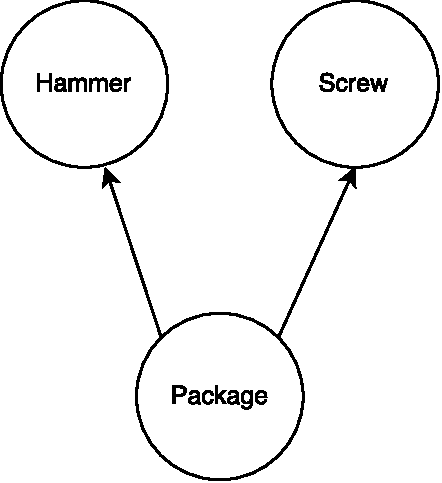
\includegraphics[width=0.3\textwidth]{dependencygraph.pdf}
\caption{Dependency graph describing order of actions}
\label{fig:dependency-graph}
\end{figure}

We also choose to not model items which have a distributed production. Distributed execution means that an item may have different parts located on different modules at the same time. Going back to the example with the doll, this could allow us to paint the arms, legs head and base of the doll before putting it all together. To simplify our model we look past this. Thus, an item can only be located at a single module at one point in time. At the CP-learning factory we see no distributed production of any item. Thus we are still able to model some real life items. This restriction also means that each modelled item may only be located at one single module at a time, it may only start on a specific module and when removed from the factory it has to be removed completely.

In UPPAAL we use the template construct to model groups of similar entities, akin to classes in object oriented programming. From each template we can create several instances. The difference from traditional classes is that templates are not only described by local functions and variables, but also a graphically designed timed automata. 

In the following we describe how we model items in our UPPAAL model through the use of the \emph{Recipe} and \emph{RecipeQueue} templates. The templates are named this way, because an item in the model is described by the order work types that need to be performed on it. Alike to a recipe in cooking. Instances of the \emph{Recipe} template are therefore known as recipes, but they do in fact model items.  

\subsection{Recipe}\label{subs:recipe}\todo{Skal de stadig kaldes recipes?}
It is possible to construct a functional dependency graph in UPPAAL using the graphical tools, creating a new template for each new item type. However, as will be revealed in \cref{ch:configuration}, we wish to be able to instantiate a factory and its ordered items through python, instead of writing directly in UPPAAL. This requires that we edit the XML file in which our model is described. Having to generate a new template from scratch for each recipe type, would be very cumbersome. Instead we create a single recipe template that, depending on its instantiating parameters, functions according to a specific functional dependency graph. Thus we only have to generate code for instantiating templates.

Our recipe template can be seen in \cref{fig:recipe}. To describe the underlying functional dependency graph, the template is instantiated with an array of nodes. The \emph{Node} struct is shown in \cref{code:Node}. This reveals that each node knows what type of work it represents, the number of parents it has, its children's indexes in the node array and the number of children. Node A is parent of node B if B depends on A and the other way around for children. In addition a recipe is also instantiated with a unique id, the id of the module it begins at, as well as the direction it enters this module from. 

\lstinputlisting[language=C, caption=Node struct, captionpos = b, label={code:Node}, float]{codeRelated/UPPAAL/node.txt}

When a recipe begins processing, it is placed onto its start module, and we find the ids of nodes, which do not depend on any other node. The ids of these are placed into the local \emph{current\_nodes} array, and represent what works can be performed on the recipe. After this, the recipe is moved along the factory. Each time it meets a module, where it wishes to have work performed, it will handshake on its own private channel with the module to identify itself. Afterwards it will synchronize with the module again on one of the allowed \emph{work} channels. A work channel can be synchronized on, if one of the nodes in the \emph{current\_nodes} array, represent the work type corresponding to that work channel. This check is done by the \emph{is\_callable} function.

Before going back to the \emph{InProgress} location, a call to \emph{update\_current\_nodes} is made. The code of this function can be seen in \cref{code:updatecurrentnodes}. It will first collect all current nodes in the \emph{new\_nodes} array, except for \emph{called\_node}, as this is the node just worked on. It then runs over each of \emph{called\_node}'s children to decrement their \emph{number\_of\_parents} field by 1. If this field reaches 0, it means that the node no longer has any dependencies and can be worked on. Because of this it is added to the \emph{new\_nodes} array. Once all children have been updated, the contents of \emph{new\_nodes} are used to update \emph{current\_nodes}.  

\lstinputlisting[language=C, caption={The update\_current\_nodes function}, captionpos = b, label={code:updatecurrentnodes}, float]{codeRelated/UPPAAL/updatecurrentnodes.txt}

After the call to \emph{update\_current\_nodes} is finished, we call \emph{no\_more\_nodes}. This will set the local \emph{done} boolean to \emph{True}, if \emph{current\_nodes} nodes is empty. This means that the recipe can not be worked on any further and may be removed.

\subsection{RecipeQueue}\label{subs:recipequeue}

\begin{figure}[h]
\centering
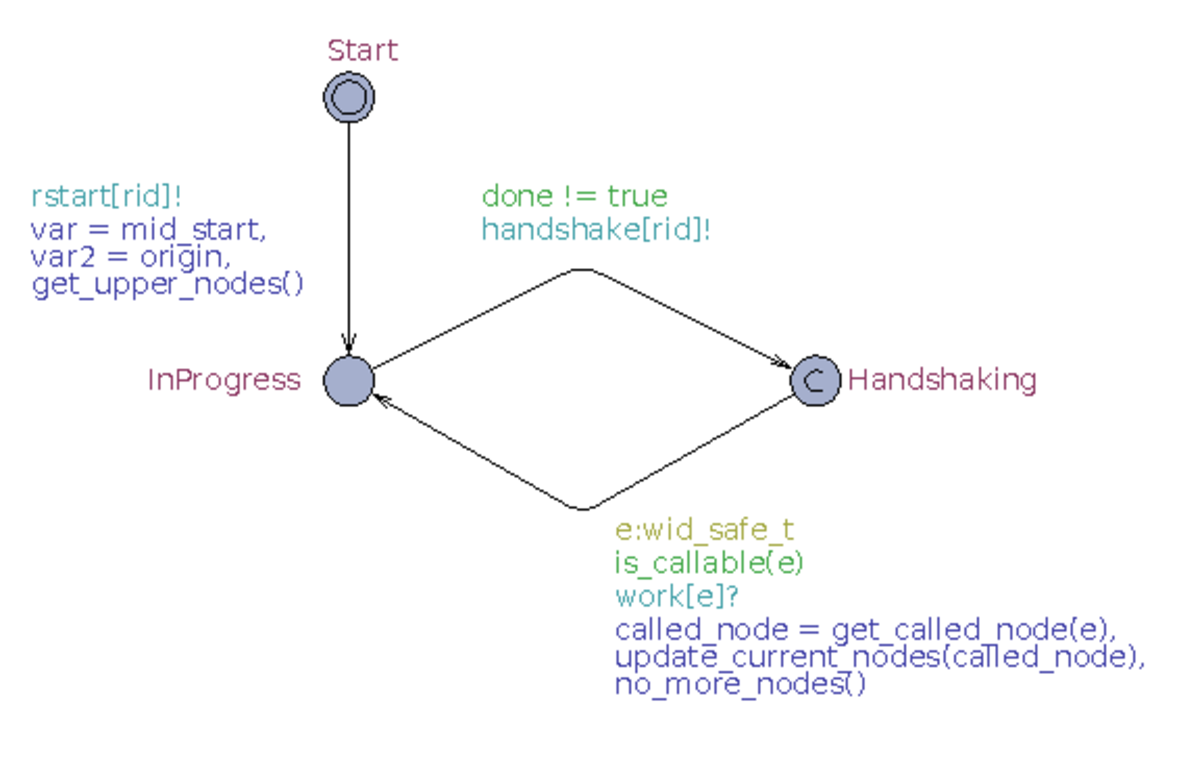
\includegraphics[width=\textwidth]{recipe.pdf}
\caption{Recipe template}
\label{fig:recipe}
\end{figure}

Having all recipe instances compete for a place on the factory leads to a large state-space, when we ask UPPAAL to find the best timed trace. In order to get around this we enforce a certain order in which recipes may be placed into the factory.  This is done using a queuing system, which we implement using the \emph{RecipeQueue} template as seen in \cref{fig:recipequeue}.

The template is instantiated with an array of recipe ids indicating the order in which we wish the recipes produced. Once instantiated, the queue may have a recipe dequeued, which may then begin processing. This reduces the state space, as recipes are to begin in a specified order. We will not get into how to produce an efficient ordering of recipes here, as it will be brought up in \cref{ch:configuration}.

\begin{figure}[h]
\centering
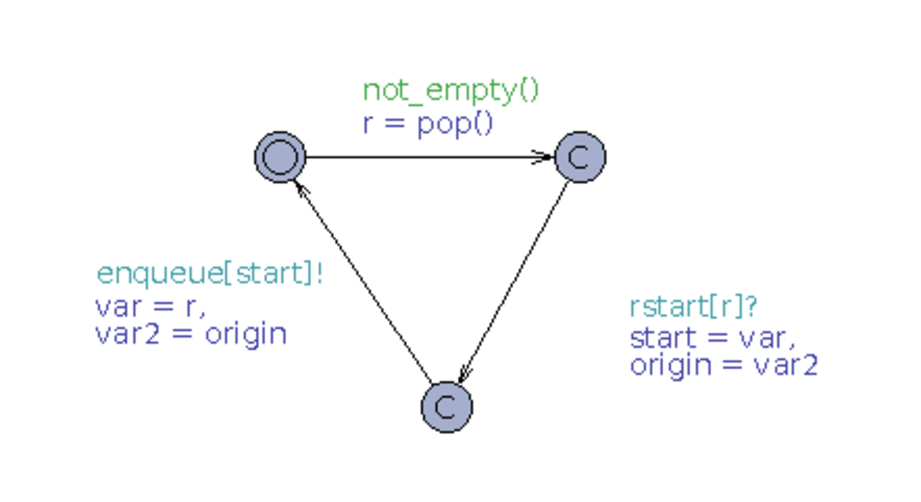
\includegraphics[width=\textwidth]{recipequeue.pdf}
\caption{RecipeQueue template}
\label{fig:recipequeue}
\end{figure}